\documentclass[pdflatex,sn-apa]{sn-jnl}

\usepackage{graphicx}%
\graphicspath{{figs/}}%
\usepackage{multirow}%
\usepackage{amsmath,amssymb,amsfonts}%
\usepackage{amsthm}%
\usepackage{mathrsfs}%
\usepackage[title]{appendix}%
\usepackage{xcolor}%
\usepackage{textcomp}%
\usepackage{manyfoot}%
\usepackage{booktabs}%
\usepackage{algorithm}%
\usepackage{algorithmicx}%
\usepackage{algpseudocode}%

\theoremstyle{thmstyleone}%
\newtheorem{theorem}{Theorem}%
\newtheorem{proposition}[theorem]{Proposition}%
\newtheorem{lemma}[theorem]{Lemma}%

\theoremstyle{thmstyletwo}%
\newtheorem{remark}{Remark}%

\theoremstyle{thmstylethree}%
\newtheorem{definition}{Definition}%
\newtheorem{assumption}{Assumption}%

\newcommand{\indep}{\perp\!\!\!\perp}
\newcommand{\Fcal}{\mathcal{F}}
\newcommand{\Scal}{\mathcal{S}}
\newcommand{\Gstar}{\mathcal{G}^{\star}}
\newcommand{\pa}{\mathrm{pa}}
\newcommand{\de}{\mathrm{de}}
\newcommand{\Prob}{\mathbb{P}}
\newcommand{\Exp}{\mathbb{E}}
\newcommand{\Real}{\mathbb{R}}

\raggedbottom

\begin{document}

\title[Certificate-Only Causal Discovery]{Certificate-Only Causal Discovery:
Monitoring-Valid Edges and Predictive-Fit Orientation}

\author*[1]{\fnm{Quang-Vinh} \sur{Dang}}\email{vinh.dq4@buv.edu.vn}

\affil*[1]{\orgname{British University Vietnam}, \orgaddress{\city{Hung Yen},
\country{Vietnam}}}

\abstract{Constraint-based causal discovery deletes an edge when a
conditional-independence test fails to reject, so a lack of power is reported
as a conclusion, and rerunning it as data arrive accumulates false edges. We
study certificate-only discovery, which asserts a feature of the graph only by
rejecting a null that is true whenever the feature is absent. The adjacency
certificate is the minimum over conditioning sets of sequential tests: a
Bayes-factor test of a partial regression coefficient (exact for Gaussian
regression errors) or a nonparametric sequential generalised covariance test that
allows nonlinear mechanisms (asymptotic). It bounds the probability that a false
edge is ever certified, uniformly over time and without faithfulness, within those
models. The orientation certificate compares sequentially fitted forecasters for
the two factorisations of a pair and reports a direction only when two model
classes agree; it certifies better predictive fit, not causation. In 150 random
graphs monitored from $n=100$ to $6400$, CERT-CD reported a false edge in $2.7\%$
of graphs under Laplace noise (off the Gaussian model), against $27\%$ to $91\%$ for
PC, GES and DirectLiNGAM and $32\%$ to $79\%$ for PC with the same nonparametric test;
its recall is low at small samples and most non-adjacent pairs stay undecided. With
nonlinear mechanisms the linear test reported a false edge in about half of the
graphs and the nonparametric test in $1$ to $2$ of $60$. On the Tübingen pairs the
orientation certificate committed on $12$ of $80$ scorable pairs and was right on
$11$, as often as the twelve most confident pairs of RECI. On $19$ untouched
recordings of physical devices with known graphs (Causal Chambers) the guarantee
did not hold: CERT-CD still reported a false edge, adjusted for dependences the
graph cannot explain, in $12$ recordings, though with the fewest false edges per
recording of the methods compared and a recall of $0.12$ to $0.25$. Both
certificates fail outside their models, and we report where.}

\keywords{causal discovery, anytime-valid inference, e-values, sequential
testing, additive noise models, family-wise error control}

\pacs[MSC Classification]{62L12, 62H22, 62F03}

\maketitle


\section{Introduction}\label{sec:intro}

A causal discovery algorithm returns a graph, and a practitioner reading it
wants to know which of its features the data support. Constraint-based methods
such as PC and FCI
\citep{spirtes2000causation,spirtes1995causal,colombo2012learning} start from
the complete graph and delete an edge whenever a conditional-independence test
fails to reject. Failure to reject is compatible with independence, with a
dependence too weak to see at the current sample size, and with a test that had
little power; the deletion happens regardless. Two consequences follow.
Finite-sample correctness requires faithfulness or a quantitative strengthening
of it \citep{robins2003uniform,uhler2013geometry}, because only such an
assumption turns ``the test did not reject'' into ``the variables are
independent''. And the output is two-valued where the evidence is three-valued:
a missing edge means either ``the data indicate no edge'' or ``nothing was
established about this pair''.

There is a third consequence that matters in practice. Data accumulate, and an
analyst who inspects the estimate as they do, and keeps any edge that has ever
appeared, is performing optional stopping. A fixed-sample guarantee does not
cover this. Section~\ref{sec:exp-monitoring} measures the effect on eight-node
graphs: when PC, GES and DirectLiNGAM are rerun at each sample size from $100$
to $6400$, between a quarter and nine tenths of the graphs have at least one
false edge in the union of the estimates.

This paper studies the opposite discipline, which we call \emph{certificate-only}
discovery: assert a feature of the graph only by rejecting a null hypothesis
that is true whenever the feature is absent, and never assert anything by
failing to reject. An algorithm that obeys the rule starts from the empty graph
and adds; it cannot report an edge as absent, only as undecided; and what it
controls is the probability of asserting something false. If each test is an
anytime-valid process, the guarantee holds at every sample size at once and
survives continuous monitoring.

\paragraph{Contributions.}

\begin{enumerate}
\item \emph{Adjacency certificates under monitoring.} For a linear structural
  equation model with independent errors, d-separation implies that a partial
  regression coefficient is zero, so adjacency has a certifying null that
  needs no faithfulness and no Gaussian errors. The minimum over conditioning
  sets of per-set sequential tests bounds the probability that a false edge is
  \emph{ever} certified (Section~\ref{sec:adjacency}). The bound is exact for
  Gaussian errors and asymptotic otherwise, and we measure how far from
  nominal it is off-model (Section~\ref{sec:exp-primitive}).
\item \emph{An orientation certificate based on predictive fit.} For a pair of
  variables we fit forecasters for the factorisations $x\to y$ and $y\to x$
  sequentially, and certify a direction when the running mean of the
  log-score difference has a confidence sequence that excludes zero under two
  model classes at once (Section~\ref{sec:orientation}). The claim is about
  predictive fit and is valid whether or not either model is correct; it
  identifies the causal direction under additive-noise models.
\item \emph{Evidence under pre-specified protocols.} We compare against PC,
  GES and DirectLiNGAM under monitoring (Section~\ref{sec:exp-monitoring}),
  evaluate the orientation certificate on simulated pairs and on the
  Tübingen cause-effect pairs with a protocol committed before the run
  (Sections~\ref{sec:exp-pairs} and~\ref{sec:exp-tuebingen}), evaluate it on physical devices with a known graph
  (Section~\ref{sec:exp-chamber}), study scaling with graph size, sample size and the constants of the algorithm
  (Sections~\ref{sec:exp-scaling} and~\ref{sec:exp-ablation}), and report the
  regimes where the certificates fail (Sections~\ref{sec:exp-pairs}
  and~\ref{sec:exp-scope}).
\end{enumerate}

\paragraph{Scope.} The method targets continuous, observational data from a
causally sufficient system whose mechanisms are linear or additive-noise, at
sample sizes of a few hundred or more. We chose the benchmarks to match this
domain and fixed the selection criteria before running; data outside it are
reported as a limitation, not dropped.

\paragraph{Outline.} Section~\ref{sec:related} places the work in the literature.
Section~\ref{sec:method} develops the certificates and the algorithm.
Section~\ref{sec:experiments} reports the experiments and
Section~\ref{sec:discussion} discusses limitations. Proofs and further results
are in the appendices.


\section{Related work}\label{sec:related}

\paragraph{Error control in constraint-based discovery.} PC-p
\citep{strobl2019estimating} bounds an edge's p-value by the maximum p-value
over conditioning sets and controls the false discovery rate of edge and
orientation decisions with Benjamini--Yekutieli; it is finite-sample but
valid at a fixed sample size, and its orientation rules operate within the
Markov equivalence class. The conservative PC algorithm of
\citet{ramsey2006adjacency} marks ambiguous triples instead of resolving them, and
\citet{li2009controlling} control the false discovery rate of the edges of PC at a fixed
sample size. We split the level over pairs by a union bound; an e-value
false-discovery-rate procedure \citep{wang2022false} would be less conservative and is
not pursued here.
Faithfulness-based guarantees break down when parameters are near a
cancellation \citep{robins2003uniform,uhler2013geometry,zhang2008detection}.
$\epsilon$-CUT \citep{shaska2025causal} gives one-sided false-edge control
without faithfulness at each fixed sample size; \citet{csillag2025prediction}
calibrate batched Fisher-$z$ statistics into per-test e-values inside PC.
The certificate-only discipline here is the same one-sided logic made
time-uniform and extended to orientation.

\paragraph{Anytime-valid inference.} Ville's inequality \citep{ville1939etude}
underlies confidence sequences \citep{darling1967confidence,robbins1970statistical,
howard2021timeuniform} and the e-value literature
\citep{vovk2021evalues,ramdas2023gametheoretic,grunwald2024safe}.
Asymptotic confidence sequences \citep{waudbysmith2024asymptotic} and
anytime-valid linear models \citep{lindon2026anytime} extend the approach to
regression coefficients under weak moment conditions, and sequential tests of
independence and conditional independence have been built from predictive
comparisons and from learned regressions
\citep{podkopaev2023sequential,waudbysmith2023sequential}. Our nonparametric primitive is
of the latter kind, built on the generalised covariance measure
\citep{shah2020hardness}, whose bias is a product of two regression errors, the
structure that debiased machine learning exploits \citep{chernozhukov2018double}
(see also \citealt{lundborg2022conditional} for conditional independence tests in
function spaces). What is new here is the use of such tests as certificates,
minimised over conditioning sets and combined into a graph. Conditional-independence
testing is intrinsically hard: no test with uniform level over all
conditional-independence nulls has power against any alternative
\citep{shah2020hardness}. Sequential tests therefore either assume a known
conditional law \citep{shaer2023model,grunwald2024modelx} or restrict the null,
as we do by testing a partial regression coefficient.

\paragraph{Orientation.} Linear non-Gaussian models identify the full graph
\citep{shimizu2006linear} and DirectLiNGAM \citep{shimizu2011directlingam} and
the pairwise likelihood ratios of \citet{hyvarinen2013pairwise} estimate it;
\citet{shimizu2008use} test direction using non-normality. Additive-noise models
\citep{hoyer2009nonlinear,peters2014identifiability} identify direction for
nonlinear mechanisms, and location-scale models extend this to heteroscedastic
noise \citep{xu2022heci,immer2023loci}. Compression- and quantile-based scores
\citep{marx2017slope,tagasovska2020bqcd} perform well on the Tübingen pairs
\citep{mooij2016distinguishing}. The marginal variances of simulated data can leak the causal order
\citep{reisach2021beware}; all our variables are standardised on a warm-up before
analysis, which removes that signal. Linear methods fit those pairs poorly
\citep{schkoda2025goodness}, and a test that is valid against a misspecified
model does not control direction error. Methods that abstain exist:
\citet{prakash2024diagnostic} and \citet{ding2025gaussdetect} return an
inconclusive outcome, \citet{prakash2026power} gate on a linearity check, and
\citet{uehara2026iterative} attach per-edge resolved or impossible codes in an
interactive protocol. None of these gives a time-uniform error statement; ours
is a statement about predictive fit that holds without either model being
correct (Section~\ref{sec:orientation}), a comparison in the spirit of
\citet{vuong1989likelihood} and of sequential forecaster comparison
\citep{choe2024comparing}.


\section{Method}\label{sec:method}

\subsection{Setting and assumptions}\label{sec:setting}

Let $\Gstar$ be a directed acyclic graph on $V=\{1,\dots,d\}$ and let
$X=(X_1,\dots,X_d)$ follow a linear structural equation model
$X = B^\top X + e$, where $B$ is supported on the edges of $\Gstar$ and the
errors $e_1,\dots,e_d$ are mutually independent with finite fourth moments.
Observations $o_1,o_2,\dots$ are i.i.d.\ draws of $X$ and arrive in batches;
$\Fcal_t$ is the $\sigma$-field of the first $t$ observations. We write
$\pa(i)$ and $\de(i)$ for the parents and descendants of $i$ and
$\Scal_k(i,j)=\{S\subseteq V\setminus\{i,j\}: |S|\le k\}$ for the admissible
conditioning sets, a family fixed before any data are seen.

\begin{assumption}[Separator size]\label{ass:sep}
Every non-adjacent pair of $\Gstar$ has a d-separating set of size at most $k$.
\end{assumption}

Assumption~\ref{ass:sep} is structural. It holds whenever $k$ is at least the
maximum in-degree of $\Gstar$, because for non-adjacent $i,j$ either
$\pa(i)$ or $\pa(j)$ d-separates them; $k=d-2$ makes it vacuous at an
exponential computational cost.

For a pair $(i,j)$ and a set $S$ let $\beta_{i\leftarrow j\cdot S}$ denote the
coefficient of $X_j$ in the population regression of $X_i$ on
$(1,X_j,X_S)$.

\begin{lemma}\label{lem:partial}
If $S$ d-separates $i$ and $j$ in $\Gstar$, then
$\beta_{i\leftarrow j\cdot S}=0$.
\end{lemma}

\noindent This is the standard fact that d-separation implies a vanishing
partial covariance in a linear structural equation model
\citep{spirtes2000causation}. It is a moment condition, weaker than
conditional independence, and it does not require Gaussian errors. Faithfulness
is the converse and is not assumed.

\subsection{Certificates}\label{sec:principle}

\begin{definition}\label{def:cert}
Let $\phi$ be a feature of $\Gstar$. A \emph{certifying null} for $\phi$ is a
hypothesis $H_\phi$ that holds whenever $\phi$ is false. A process
$(E_t)_{t\ge 0}$ is \emph{Ville-valid} for $H$ if $E_t\ge 0$ and
$\Prob(\exists t: E_t\ge\lambda)\le 1/\lambda$ for every $\lambda\ge 1$ and every
$P\in H$. A \emph{certificate for $\phi$ at level $\alpha$} is the event that a
Ville-valid process for $H_\phi$ reaches $1/\alpha$.
\end{definition}

\begin{proposition}[Soundness]\label{prop:single}
If $\phi$ is false, the probability that it is ever certified at level
$\alpha$ is at most $\alpha$.
\end{proposition}

\noindent The proof is the definition: if $\phi$ is false then $P\in H_\phi$.
The implication runs one way. $H_\phi$ may also hold when $\phi$ is true, and
the certificate then never fires; this is what buys validity without
faithfulness and what costs power. Three consequences follow. There is no
certifying null for ``$i$ and $j$ are non-adjacent'', so the algorithm cannot
delete and must start from the empty graph. Its output is three-valued
(certified adjacent, certified with a direction, undecided). And power is
descriptive: nothing guarantees that a true edge is ever certified.

\emph{Ville-valid} is weaker than \emph{e-process}, which requires
$\Exp[E_\tau]\le 1$ at every stopping time of a single filtration. All our
bounds use only the event that a process ever reaches a level, so they hold at
every data-dependent stopping time of the run, but we do not claim the
stronger property. Section~\ref{sec:primitive} shows why.

\subsection{The adjacency certificate}\label{sec:adjacency}

For a pair $(i,j)$ consider
\begin{equation}\label{eq:sepnull}
H^{\mathrm{sep}}_{ij}:\quad \exists S\in\Scal_k(i,j)\ \text{ with }\
\beta_{i\leftarrow j\cdot S}=0 .
\end{equation}
By Lemma~\ref{lem:partial} and Assumption~\ref{ass:sep}, $H^{\mathrm{sep}}_{ij}$
holds for every non-adjacent pair, so it is a certifying null for adjacency.
Let $E^{(S)}_t$ be a Ville-valid process for the point null
$\beta_{i\leftarrow j\cdot S}=0$ and define
\begin{equation}\label{eq:adjacency}
A_t(i,j)=\min_{S\in\Scal_k(i,j)} E^{(S)}_t(i,j).
\end{equation}

\begin{proposition}\label{prop:adjacency}
Let $\lambda\ge 1$ and let $(i,j)$ be non-adjacent. Then
$\Prob(\exists t: A_t(i,j)\ge\lambda)\le 1/\lambda$.
\end{proposition}

\begin{proof}
Choose $S^\star\in\Scal_k(i,j)$ with $\beta_{i\leftarrow j\cdot S^\star}=0$.
Since $A_t\le E^{(S^\star)}_t$ pointwise, the event $\{\exists t:A_t\ge\lambda\}$
is contained in $\{\exists t:E^{(S^\star)}_t\ge\lambda\}$, which has probability
at most $1/\lambda$.
\end{proof}

\noindent That the minimum of e-values is an e-value for a union null is
standard \citep{vovk2021evalues}; the proof above needs only the inclusion of
events, so the processes $E^{(S)}$ may live in different filtrations. Faithfulness enters only through power: adjacency-faithfulness makes every
$E^{(S)}$ grow for a genuinely adjacent pair, and an instance where it fails
leaves the pair undecided instead of producing a wrong edge.

\subsubsection{The per-set primitive}\label{sec:primitive}

For $S$ with $|S|=q-1$ write the regression
$X_i=\alpha^\top(1,X_S)+\beta X_j+\varepsilon$ and let $S_{ii},S_{ij},S_{jj}$
be the cross-products of the residuals of $X_i$ and $X_j$ after regression on
$(1,X_S)$, computed from the running Gram matrix of the centred data, with
$p=|S|+1$. With a right-Haar prior on the nuisance parameters and
$\beta\mid\sigma\sim N(0,\sigma^2 g)$ for a fixed $g>0$, the Bayes factor is
\begin{equation}\label{eq:safelinear}
E_n=(1+G)^{-1/2}\bigl(1-\kappa\,\hat r_n^2\bigr)^{-(n-p)/2},\qquad
G=g\,S_{jj},\quad \kappa=\tfrac{G}{1+G},\quad
\hat r_n^2=\tfrac{S_{ij}^2}{S_{ii}S_{jj}}.
\end{equation}
It depends on the data only through Schur complements of the Gram matrix, so a
single $O(d^2)$ statistic serves every hypothesis $(i,j,S)$. The prior scale
$g$ must be fixed before the data: a $g$ that adapts to the running sample size
destroys the martingale property. We fix it in advance and use a warm-up prefix,
discarded from every process, only to standardise the variables.

\begin{proposition}\label{prop:safelinear}
Suppose $\varepsilon\sim N(0,\sigma^2)$ is independent of $(X_j,X_S)$ and
$\beta=0$. Then $(E_n)$ is a non-negative martingale with mean one in the
filtration generated by the sequence of maximal invariants of the nuisance group
(translations in the span of $(1,X_S)$ and rescaling of $X_i$), and therefore
$\Prob(\exists n: E_n\ge\lambda)\le 1/\lambda$ for every $\lambda\ge1$.
\end{proposition}

\noindent The proof is the right-Haar argument of
\citet{hendriksen2021optional} and \citet{grunwald2024safe} and is given in
Appendix~\ref{app:safelinear}. The regressors may have any distribution;
Gaussianity is required of the regression error $\varepsilon$, which for
$S\supseteq\pa(i)$ with no descendant of $i$ is the structural error $e_i$.

\begin{remark}[The raw-observation filtration]\label{rem:raw}
$(E_n)$ is \emph{not} a martingale in the filtration generated by the raw
observations. With $S=\emptyset$, $g=0.25$ and
$X_{1:2}=Y_{1:2}=(-1,1)$, Eq.~\eqref{eq:safelinear} gives $E_2=1$ while
$\Exp[E_3\mid\Fcal_2]=1.083>1$ under an i.i.d.\ standard Gaussian null (numerical
integration). Amenability of the nuisance group does not repair this. The
guarantee used here, a bound on the probability of ever crossing, does not need
the raw filtration, which is why Proposition~\ref{prop:adjacency} was stated for
events.
\end{remark}

\begin{remark}[Role averaging]\label{rem:avg}
Eq.~\eqref{eq:safelinear} treats $X_i$ as the response, and the roles of $i$
and $j$ are interchangeable under the null. The implementation averages the two
role-swapped Bayes factors to remove the arbitrary choice. A crossing of the
average implies a crossing of one of the two, each of probability at most
$1/\lambda$, so the guaranteed bound for the averaged process is $2/\lambda$.
\end{remark}

\begin{remark}[Beyond Gaussian errors]\label{rem:offmodel}
When the regression error is not Gaussian, or its variance depends on the
regressors, Eq.~\eqref{eq:safelinear} is the $d=1$ case of the model-based
test of \citet{lindon2026anytime}, whose guarantee under the moment null
$E[W\varepsilon]=0$ is asymptotic and holds when the model variance equals the
heteroscedasticity-robust variance. A robust sandwich version exists
\citep[Theorem~5.4 of the arXiv version]{lindon2026anytime}. Finite-sample
validity over all finite-variance laws is impossible without tail control
\citep{shah2020hardness}. We therefore state the adjacency guarantee as
\emph{exact for Gaussian regression errors and asymptotic otherwise}, and
Section~\ref{sec:exp-primitive} measures the finite-sample departure under
heavy tails and heteroscedasticity for both versions.
\end{remark}

\begin{remark}[One model for both certificates]\label{rem:common}
Both certificates live in the linear structural equation model with
independent errors. Adjacency uses only second moments, through
Lemma~\ref{lem:partial}; orientation uses the shape of the error laws and, in
the additive-noise extension, nonlinear mechanisms, for identifiability only.
The validity statement of the orientation certificate
(Section~\ref{sec:orientation}) does not depend on either error law.
\end{remark}

\subsection{The orientation certificate}\label{sec:orientation}

Fix a pair $(x,y)$. For each direction we fit a forecaster of the joint law on
the past and score it on the next observation. Let
$p^{x\to y}_s$ be the density of the forecaster for the factorisation
$p(x)\,p(y\mid x)$ fitted on observations $1,\dots,s-1$ and $p^{y\to x}_s$ the
mirror forecaster, and set
\begin{equation}\label{eq:increment}
d_s=\log p^{x\to y}_s(x_s,y_s)-\log p^{y\to x}_s(x_s,y_s).
\end{equation}
Both forecasters are $\Fcal_{s-1}$-measurable, and both are densities on the
same space, so $d_s$ is a legitimate score difference whether or not either
model is correct. Let $\bar\mu_t=t^{-1}\sum_{s\le t}\Exp[d_s\mid\Fcal_{s-1}]$
and let $\hat\mu_t$ and $\hat\sigma_t$ be the running mean and standard
deviation of $(d_s)$. The confidence sequence of
\citet[Theorem~2.2]{waudbysmith2024asymptotic} is
\begin{equation}\label{eq:csd}
\hat\mu_t\pm\hat\sigma_t\sqrt{\frac{2(t\rho^2+1)}{t^2\rho^2}
\log\frac{\sqrt{t\rho^2+1}}{\alpha}},
\end{equation}
with $\rho$ tuned to a reference time $t^\ast=200$. We certify $x\to y$ at the
first $t$ at which the lower end exceeds zero and $y\to x$ when the upper end
falls below zero; both are decided only after $60$ scored observations.

\begin{proposition}\label{prop:orient}
Let $\Fcal_{s-1}$ be the past, let the forecasters be $\Fcal_{s-1}$-measurable,
and suppose the martingale differences $d_s-\Exp[d_s\mid\Fcal_{s-1}]$ satisfy
the moment conditions of \citet[Theorem~2.2]{waudbysmith2024asymptotic}. Then
\eqref{eq:csd} is an asymptotic confidence sequence for $\bar\mu_t$ at level
$1-\alpha$. In particular, if $y\to x$ predicts at least as well as $x\to y$
on average ($\bar\mu_t\le 0$ for all $t$), the probability of ever certifying
$x\to y$ is at most $\alpha$ asymptotically.
\end{proposition}

\noindent What is certified is therefore that one factorisation has a
strictly better expected log score, and this is valid without either
forecaster being correct. It corresponds to the causal direction under the
identifiability results for additive-noise models
\citep{hoyer2009nonlinear,peters2014identifiability} and for linear
non-Gaussian models \citep{shimizu2006linear}: if the data come from
$x\to y$, the true class is contained in the forecaster family and the
estimates are consistent, the expected score of the correct factorisation
exceeds that of the reversed one by a positive Kullback--Leibler gap, because
for generic mechanisms or non-Gaussian errors the reversed factorisation cannot
represent the joint law. Under confounding or selection the better predictor
need not be the cause, and the certificate then says nothing about causation.
The conclusion of Proposition~\ref{prop:orient} is asymptotic, and
Section~\ref{sec:exp-pairs} reports its finite-sample behaviour.

\paragraph{Forecasters.} Both use a generalised-Gaussian density
$g(u)\propto\exp(-|u/s|^\kappa)$ with shape $\kappa\in[0.9,8]$ fitted by
maximum likelihood, a generalised-Gaussian marginal for the cause, and a
cubic truncated-power spline mean with four quantile knots, set from the
warm-up prefix, for the effect. The class \texttt{gg} has constant scale; the
class \texttt{ggh} lets the log-scale be quadratic in the cause, which covers
heteroscedastic noise
\citep{xu2022heci,immer2023loci}. The \emph{agreement} certificate reports a
direction only when both classes certify the same one. Each class is
Ville-bounded by the same argument, so agreement cannot err more often than
either alone; its purpose is protection against model-class mistakes: the
constant-scale class alone certifies the wrong direction on every
heteroscedastic Gaussian pair it decides in our simulations, and the location-scale class alone is too
flexible to resolve linear non-Gaussian pairs
(Section~\ref{sec:exp-pairs}). Preprocessing is fixed in advance: tied values
are dequantised, the order is randomly permuted, and $\max(100,\lceil0.2n\rceil)$
observations form a warm-up prefix used for standardisation and knots.

\subsection{The algorithm and its guarantee}\label{sec:algorithm}

CERT-CD maintains a three-valued state for every pair. It streams data in
batches, updates the running Gram matrix, recomputes $A_t(i,j)$ for every
undecided pair, and certifies adjacency when $A_t(i,j)$ crosses its threshold.
The total budget is split as $\alpha=\alpha_A+\alpha_D$, with $\alpha_A$ spread
over the $\binom d2$ adjacency nulls and $\alpha_D$ over the direction nulls,
and the thresholds are $\lambda_A=\binom d2/\alpha_A$ and
$\lambda_D=d(d-1)/\alpha_D$, fixed before the data arrive. Which pairs are
examined does not enter the bound.

\begin{theorem}[Adjacency]\label{thm:main}
Under Assumption~\ref{ass:sep}, linear structural equations with independent
errors, and Gaussian regression errors in~\eqref{eq:safelinear} for every
examined $(i,j,S)$, the probability that CERT-CD ever certifies an edge between
a non-adjacent pair is at most $2\alpha_A$, uniformly over time and at every
data-dependent stopping time of the run.
\end{theorem}

\begin{proof}
By Remark~\ref{rem:avg} each pair's averaged minimum has crossing probability at
most $2/\lambda_A$ by Proposition~\ref{prop:adjacency}. A union bound over at
most $\binom d2$ non-adjacent pairs gives $\binom d2\cdot 2/\lambda_A=2\alpha_A$.
\end{proof}

\noindent Choosing $\lambda_A=2\binom d2/\alpha_A$ gives $\alpha_A$ exactly; the
experiments use the shipped threshold, so the guaranteed bound there is
$2\alpha_A$. Under non-Gaussian errors the bound holds asymptotically
(Remark~\ref{rem:offmodel}). The orientation layer inside the multivariate
algorithm uses a linear generalised-Gaussian universal-inference certificate
whose validity is conditional on the model describing each pair given a block
of conditioning variables frozen when the edge is certified
(Appendix~\ref{app:linear}); the relative-fit certificate of
Section~\ref{sec:orientation} is bivariate and is evaluated on pairs. An
extension that conditions the relative-fit forecasters on the frozen block is
possible but not evaluated here.


\section{Experiments}\label{sec:experiments}

\subsection{Protocol}\label{sec:protocol}

The benchmarks were chosen to match the scope of the method: continuous data,
linear or additive-noise mechanisms, a few hundred observations or more. The
protocols of the monitoring experiment, the Tübingen evaluation, the simulations
of the orientation certificate and of the primitive off the Gaussian model, the
held-out pair families and the scaling and nonlinear experiments were written and
committed to the repository before the runs. The two exceptions are the
redesign evaluated on the Causal Chambers (Section~\ref{sec:exp-chamber}) and the
nine design families of Section~\ref{sec:exp-pairs}, which are flagged where they
appear. The baselines IGCI, RECI, ANM-HSIC and the pairwise LiNGAM rule are our
re-implementations of the published rules (Appendix~\ref{app:extra}), and PC, GES
and DirectLiNGAM are the \texttt{causal-learn} implementations with default
settings. Data outside the scope are reported in Section~\ref{sec:exp-scope}.

\subsection{False edges under monitoring}
\label{sec:exp-monitoring}

We drew $150$ random DAGs on $d=8$ nodes (edge probability $0.25$,
coefficients with absolute value in $[0.5,1.2]$) with Laplace and with Gaussian
errors, and ran each method on nested prefixes of $n=100,200,400,\dots,6400$
observations. A graph counts as a failure if any prefix's estimate contains an
edge that is absent from the true skeleton, which is what an analyst who keeps
every edge ever seen would report. CERT-CD ran as one stream with
$\alpha=0.1$ (so $\alpha_A=0.05$ and a guaranteed bound of $0.1$ in the
Gaussian model), $k=2$, warm-up of $50$ rows and batches of $100$. The
comparators were PC (Fisher-$z$, $\alpha=0.05$ and $0.01$, \texttt{causal-learn}
defaults), GES with the BIC score, and DirectLiNGAM with edges thresholded at
$|B|>0.05$, each rerun at every $n$.

\begin{table}[t]
\caption{Probability that a false edge is ever reported over the grid
$n=100,\dots,6400$ in $150$ random eight-node graphs (Wilson $95\%$ interval for
CERT-CD only).}\label{tab:monitoring}
\begin{tabular}{@{}lcc@{}}
\toprule
Method & Laplace errors & Gaussian errors\\
\midrule
CERT-CD & $0.027$ $[0.010,0.067]$ & $0.040$ $[0.018,0.085]$\\
PC, $\alpha=0.05$ & $0.747$ & $0.773$\\
PC, $\alpha=0.01$ & $0.267$ & $0.320$\\
GES-BIC & $0.913$ & $0.960$\\
DirectLiNGAM & $0.760$ & $1.000$\\
\bottomrule
\end{tabular}
\end{table}

CERT-CD reported a false edge in $4$ of $150$ graphs under Laplace errors and in
$6$ of $150$ under Gaussian errors, against between $27\%$ and $100\%$ for the
comparators (Table~\ref{tab:monitoring}, Figure~\ref{fig:monitoring}). PC at $\alpha=0.01$ is close to a Bonferroni correction across the seven looks
($0.05/7\approx0.007$) and still reports a false edge in $27\%$ and $32\%$ of the
graphs. The comparison is deliberately about
monitoring: at a single sample size the comparators' false-edge rates are much
lower, for example $42$ of $150$ graphs for PC at $\alpha=0.05$ and $n=6400$ under
Laplace errors, so the gap is largely the cost of re-looking, which CERT-CD's
guarantee absorbs. The cost is coverage. At $n=6400$ under Laplace errors
CERT-CD's precision is $0.994$ and its recall $0.938$ ($F_1=0.965$), and it
leaves $76.8\%$ of the pairs undecided because it never certifies absence
(Gaussian: $76.9\%$). By comparison, PC at $\alpha=0.01$ has $F_1=0.970$ at the
final sample size. CERT-CD's orientation is switched on by default here, which
splits the budget; edges, not arrowheads, are scored.

\paragraph{The nonparametric certificate on the same data.} We reran the
nonparametric primitive of Section~\ref{sec:npprimitive} ($k=2$, same level) on
exactly the same $150$ DAGs and prefixes. It reported a false
edge at some sample size in $9$ of $150$ graphs under Laplace errors
($0.060$, Wilson $[0.032,0.110]$) and $7$ of $150$ under Gaussian errors
($0.047$, $[0.023,0.093]$), against $4$ and $6$ for the linear primitive. Both
are consistent with the level $\alpha_A=0.05$; the difference between the two
($9$ against $4$ under Laplace errors, $7$ against $6$ under Gaussian errors) is
within sampling noise. Its skeleton precision and recall at
$n=6400$ are $0.988$ and $0.933$ under Laplace errors
($0.990$ and $0.932$ under Gaussian), and it has no recall at $n=100$ (the
first rows are used to fit the regressions) and $0.05$ at $n=200$ under Laplace
errors, against $0.21$ and $0.65$ for the linear primitive. For graph sizes
$d=4,8,12,16$ (the scaling data below) it gives $0/60$, $3/60$, $2/60$ and $5/60$
graphs with a false edge, with precision $\ge0.992$ and recall between $0.91$ and
$0.95$.

\paragraph{Deleting with the same test.} To separate the effect of the test from the
effect of the architecture, we ran PC (depth $\le3$) with the same nonparametric
conditional-independence test used as PC uses a test: at each prefix an edge is
deleted when some conditioning set gives a $p$-value above $\alpha$ (cross-fitted
residuals, three products, Bonferroni over the three). On the same $150$ DAGs it
reported a false edge at some sample size in $115$ of $150$ graphs at
$\alpha=0.05$ ($0.767$, Wilson $[0.693,0.827]$) and $58$ of $150$ at $\alpha=0.01$
($0.387$, $[0.312,0.467]$) under Laplace errors, and in $118$ and $48$ of $150$
under Gaussian errors ($0.787$ and $0.320$). At $n=6400$ under Laplace errors its
precision and recall are $0.932$ and $0.963$ at $\alpha=0.05$ and $0.974$ and
$0.954$ at $\alpha=0.01$. The monitoring failure of the comparators is therefore
not due to the Fisher-$z$ test or to a particular score: it follows from
re-evaluating a delete-on-non-rejection procedure at each sample size.

\begin{figure}[t]
\centering
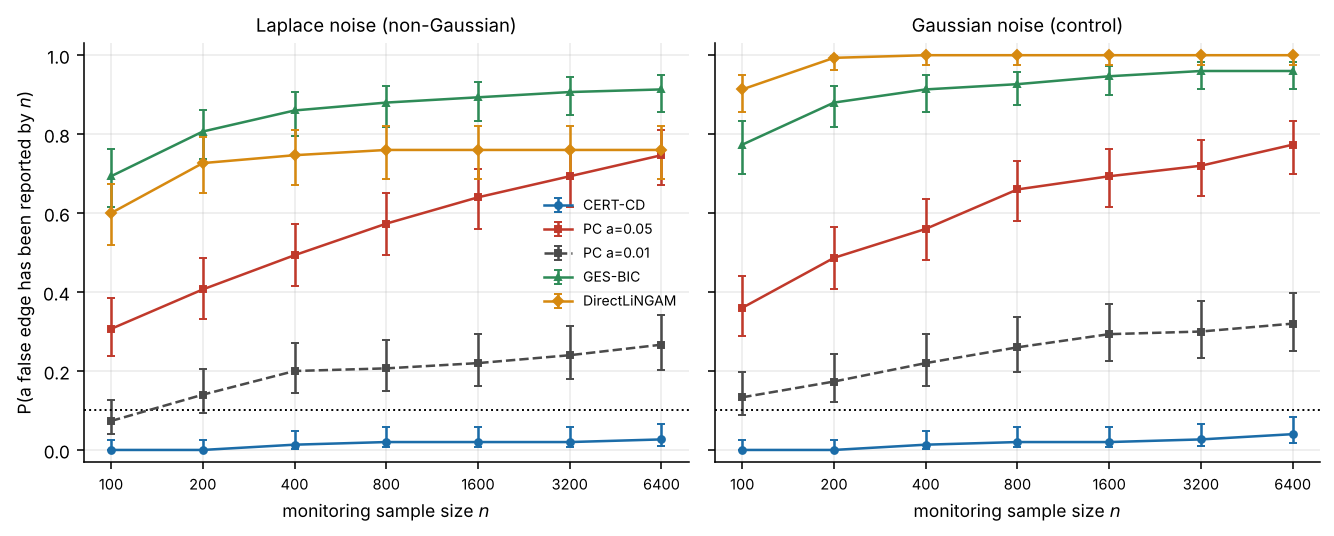
\includegraphics[width=\linewidth]{exp13_monitoring_fwer.png}
\caption{Cumulative fraction of graphs with a false edge, by sample size, for
each method (Laplace and Gaussian errors).}\label{fig:monitoring}
\end{figure}

\subsection{Sample size and graph size}\label{sec:exp-scaling}

\paragraph{Power by sample size.} The same runs give precision and recall of the
skeleton at each prefix (Table~\ref{tab:byn}, Laplace errors; under Gaussian errors
the numbers are similar except for DirectLiNGAM, whose precision is $0.61$ to $0.64$
at every $n$). CERT-CD's precision is at least $0.99$ at every $n$, but its recall
is low where the sample is small: $0.21$ at $n=100$ and $0.65$ at $n=200$,
rising to $0.94$ at $n=6400$. The comparators recover most edges from $n=100$
and pay with false edges. Under Laplace errors and at a fixed large sample DirectLiNGAM is better
than CERT-CD (precision and recall $1.00$ at $n=6400$ against
$0.99$ and $0.94$), because it uses the non-Gaussianity of every variable at
once; the claim of CERT-CD is about monitoring, not about accuracy at a single
sample size.

\begin{table}[t]
\caption{Skeleton precision / recall by sample size, Laplace errors, $150$ DAGs
at each sample size.}\label{tab:byn}
\small
\scriptsize\setlength{\tabcolsep}{2pt}
\begin{tabular}{@{}lccccccc@{}}
\toprule
$n$ & 100 & 200 & 400 & 800 & 1600 & 3200 & 6400\\
\midrule
CERT-CD & 1.00/0.21 & 1.00/0.65 & 1.00/0.82 & 1.00/0.87 & 0.99/0.91 & 0.99/0.93 & 0.99/0.94\\
PC $\alpha=0.01$ & 0.99/0.78 & 0.98/0.85 & 0.98/0.89 & 0.99/0.92 & 0.99/0.94 & 0.99/0.95 & 0.99/0.96\\
PC $\alpha=0.05$ & 0.94/0.83 & 0.95/0.87 & 0.96/0.90 & 0.96/0.93 & 0.96/0.94 & 0.96/0.95 & 0.95/0.96\\
GES-BIC & 0.83/0.93 & 0.84/0.94 & 0.87/0.96 & 0.88/0.97 & 0.92/0.98 & 0.94/0.98 & 0.94/0.99\\
DirectLiNGAM & 0.85/0.98 & 0.91/0.99 & 0.97/1.00 & 0.98/1.00 & 0.99/1.00 & 0.99/1.00 & 1.00/1.00\\
\bottomrule
\end{tabular}
\end{table}

\paragraph{Graph size.} We repeated the monitoring experiment for
$d=4,8,12,16$ with $60$ DAGs per size, Laplace errors, expected degree about
$1.75$ (realised mean degree between $1.4$ and $1.8$) and the grid $n=100,\dots,3200$ (Table~\ref{tab:scaling}). The
probability that CERT-CD ever reports a false edge is $0$, $0.050$, $0.067$ and
$0.083$, rising with $d$ but inside the guaranteed bound of $0.1$ (which is exact
only for Gaussian regression errors); the Wilson upper limit at $d=16$ is
$0.18$, so $60$ graphs cannot separate this from the bound. For PC at
$\alpha=0.05$, GES and DirectLiNGAM the probability rises to between $0.88$ and
$1.00$ at $d=12$ to $16$, and for PC at $\alpha=0.01$ to $0.67$. CERT-CD's recall
stays between $0.92$ and $0.96$, its precision above $0.99$, and the fraction
of pairs left undecided grows with $d$ ($0.56$ at $d=4$, $0.89$ at $d=16$),
because the share of non-adjacent pairs grows and none of them is ever
certified absent. The median runtime of one run at $n=3200$ is $17$, $45$, $67$
and $94$ seconds, against under three seconds for each comparator.

\begin{table}[t]
\caption{Monitoring by graph size ($60$ DAGs per size, Laplace errors,
$n\le3200$): probability of ever reporting a false edge, with the upper end of CERT-CD's
Wilson interval.}\label{tab:scaling}
\small
\scriptsize\setlength{\tabcolsep}{2pt}
\begin{tabular}{@{}lcccc@{}}
\toprule
Method & $d=4$ & $d=8$ & $d=12$ & $d=16$\\
\midrule
CERT-CD & 0.000 & 0.050 & 0.067 & 0.083\\
\quad Wilson upper limit & 0.06 & 0.14 & 0.16 & 0.18\\
PC, $\alpha=0.05$ & 0.233 & 0.667 & 0.883 & 1.000\\
PC, $\alpha=0.01$ & 0.033 & 0.267 & 0.367 & 0.667\\
GES-BIC & 0.317 & 0.933 & 1.000 & 1.000\\
DirectLiNGAM & 0.217 & 0.867 & 0.967 & 1.000\\
\midrule
CERT-CD recall at $n=3200$ & 0.964 & 0.930 & 0.922 & 0.919\\
\bottomrule
\end{tabular}
\end{table}

\subsection{Ablation of CERT-CD}\label{sec:exp-ablation}

We varied one constant at a time on $20$ eight-node DAGs with Laplace errors
($n\le3200$, same monitoring criterion; Table~\ref{tab:ablation}).

\begin{table}[t]
\caption{Ablation, $20$ DAGs, $d=8$, Laplace errors, monitored to
$n=3200$. Default: $k=2$, prior scale $0.5$, $\alpha=0.1$, orientation on.
Precision and recall are of the skeleton at $n=3200$.}\label{tab:ablation}
\small
\begin{tabular}{@{}lcccc@{}}
\toprule
Variant & ever false edge & precision & recall & median seconds\\
\midrule
default & 0/20 & 1.000 & 0.934 & 53\\
$k=0$ & 20/20 & 0.526 & 1.000 & 145\\
$k=1$ & 15/20 & 0.873 & 0.960 & 70\\
$k=3$ & 0/20 & 1.000 & 0.921 & 53\\
no orientation & 0/20 & 1.000 & 0.934 & 0.1\\
prior scale $0.25$ & 0/20 & 1.000 & 0.934 & 52\\
prior scale $1.0$ & 0/20 & 1.000 & 0.927 & 52\\
$\alpha=0.05$ & 0/20 & 1.000 & 0.927 & 53\\
$\alpha=0.2$ & 1/20 & 0.993 & 0.934 & 56\\
\bottomrule
\end{tabular}
\end{table}

The order $k$ is the only constant that matters for validity. With $k=0$ and
$k=1$, below the maximal in-degree of many of these graphs, the separator-size
assumption is violated and false edges appear in every graph ($20/20$) and in
$15/20$ respectively, with precision $0.53$ and $0.87$; with $k=3$ nothing
changes relative to $k=2$ except a slightly lower recall. The prior scale and the
total level change recall by less than $0.01$ and leave the number of graphs
with a false edge at zero, except that $\alpha=0.2$ gave one. Switching off
orientation leaves the skeleton unchanged, as it should, since the adjacency
certificates do not depend on it, and removes nearly all of the computing time:
the adjacency certificates alone take about a tenth of a second per run, and the
orientation processes dominate the cost.

\subsection{Nonlinear mechanisms}\label{sec:exp-nonlinear}

The linear primitive assumes linear mechanisms. We generated random DAGs
($d=8$, edge probability $0.25$, $60$ per cell, $n\le3200$) in which every edge
carries a nonlinear function drawn from $\{x,\tanh 2x,\sin 1.5x,x^2-1,|x|-0.8\}$,
with Laplace or Gaussian errors, and a linear control. The
linear primitive reports a false edge at some sample size in $33$ of $60$ graphs
under Laplace errors and $28$ of $60$ under Gaussian errors; the nonparametric
primitive in $1$ of $60$ (Wilson $[0.003,0.089]$) and $2$ of $60$
($[0.009,0.114]$), and it finds more of the true edges (recall $0.83$ against
$0.66$ under Laplace errors, $0.97$ against $0.62$ under Gaussian errors; precision
$0.997$ and $0.995$ against $0.83$ and $0.85$). In the linear control the two
primitives agree (false edges in $3$ and $4$ of $60$ graphs under Laplace errors,
$3$ and $3$ under Gaussian errors; recall $0.93$ against $0.92$; Table~\ref{tab:nonlinear}).

\begin{table}[t]
\caption{Nonlinear mechanisms, $60$ DAGs per row, $d=8$, $n\le3200$: graphs with a
false edge at some sample size, and skeleton precision / recall at $n=3200$.}
\label{tab:nonlinear}
\small
\begin{tabular}{@{}llcccc@{}}
\toprule
 & & \multicolumn{2}{c}{linear primitive} & \multicolumn{2}{c}{nonparametric}\\
Mechanisms & Errors & ever false & P / R & ever false & P / R\\
\midrule
nonlinear & Laplace & 33 & 0.83 / 0.66 & 1 & 0.997 / 0.83\\
nonlinear & Gaussian & 28 & 0.85 / 0.62 & 2 & 0.995 / 0.97\\
linear & Laplace & 3 & 0.99 / 0.93 & 4 & 0.99 / 0.92\\
linear & Gaussian & 3 & 0.99 / 0.93 & 3 & 0.99 / 0.93\\
\bottomrule
\end{tabular}
\end{table}

\subsection{Calibration of the adjacency primitive}
\label{sec:exp-primitive}

\paragraph{Cost and benefit of the sequential test.} With $2000$ replications
under the independence null and monitoring up to $n=1000$, a Fisher-$z$ test
inspected at every sample size falsely rejects in $34.6\%$ of runs at nominal
$\alpha=0.05$ ($56.5\%$ at $0.10$, $81.6\%$ at $0.20$; $10.0\%$ at $0.01$). The
same test at one fixed $n$ rejects $5.6\%$ ($0.01$: $1.0\%$), and the e-process
$2.4\%$ ($0.01$: $0.7\%$). The e-process is conservative by about a factor of two
at $\alpha\ge0.05$ (a factor of $1.4$ at $0.01$) in this setting, which is the cost
of the time-uniform guarantee.

\paragraph{Off the Gaussian model.} The primitive is exact only for Gaussian
regression errors. Table~\ref{tab:offmodel} reports the realised probability
of ever crossing $1/\alpha$ over $n=50,\dots,1000$ (monitored at every
observation), with $1000$ replications per cell, for a null pair with no
covariate effect (S0), a chain $i\leftarrow k\leftarrow j$ tested given $k$, and
a heteroscedastic null, under four error laws. A robust $t$-statistic
confidence sequence \citep{lindon2026anytime} is shown for comparison. For
Gaussian and Laplace errors without heteroscedasticity the primitive stays
below nominal. For skewed or heavy-tailed errors without
heteroscedasticity it is up to $2.5$ times nominal at $\alpha=0.01$ ($0.025$ for
lognormal errors), and under heteroscedastic errors it is $2.5$ to $3.2$ times
nominal at $\alpha=0.01$ and exceeds nominal at $\alpha=0.05$ for Gaussian
($0.069$) and Laplace ($0.065$) errors. The robust version is not uniformly
better: it is closer to nominal under heteroscedastic Gaussian and Laplace errors
but not under heteroscedastic $t_{2.5}$ and lognormal errors, and it is further
from nominal in the heavy-tailed homoscedastic cells ($0.098$ at $\alpha=0.05$ for
lognormal errors in S0). A separate calibration under six error laws with
homoscedastic errors ($2000$ replications, $n\le800$, Appendix~\ref{app:extra})
found every cell below nominal, the largest realised-to-nominal ratio being $0.95$
and the median about $0.48$. We therefore treat the adjacency bound of the linear
primitive as exact in the Gaussian model with homoscedastic errors and as an
approximation otherwise, with a departure that is visible under heteroscedasticity
and heavy tails.

\begin{table}[t]
\caption{Realised probability of ever crossing, $n=50,\dots,1000$ monitored every
observation (primitive, $g=0.25$) versus a robust-$t$ sequence checked every five
observations, $1000$ replications per cell.}\label{tab:offmodel}
\small
\begin{tabular}{@{}llcccc@{}}
\toprule
Scenario & Errors & BF $.05$ & BF $.01$ & robust-$t$ $.05$ & robust-$t$ $.01$\\
\midrule
S0 & Gaussian & 0.023 & 0.006 & 0.044 & 0.009\\
S0 & Laplace & 0.016 & 0.004 & 0.032 & 0.009\\
S0 & $t_{2.5}$ & 0.035 & 0.019 & 0.067 & 0.021\\
S0 & lognormal & 0.043 & 0.025 & 0.098 & 0.035\\
Chain & Gaussian & 0.021 & 0.008 & 0.042 & 0.012\\
Chain & Laplace & 0.018 & 0.006 & 0.040 & 0.011\\
Chain & $t_{2.5}$ & 0.026 & 0.013 & 0.076 & 0.035\\
Chain & lognormal & 0.039 & 0.019 & 0.086 & 0.026\\
Het. & Gaussian & 0.069 & 0.025 & 0.066 & 0.022\\
Het. & Laplace & 0.065 & 0.028 & 0.053 & 0.017\\
Het. & $t_{2.5}$ & 0.042 & 0.025 & 0.077 & 0.035\\
Het. & lognormal & 0.061 & 0.032 & 0.089 & 0.037\\
\bottomrule
\end{tabular}
\end{table}

\subsection{Graphs that violate strong faithfulness}\label{sec:exp-faith}

We generated random linear structural models with Laplace errors ($d=5$, edge
probability $0.35$, $n$ up to $3000$) until $1000$ graphs satisfied
$\delta$-strong faithfulness ($\delta=0.15$) and $500$ did not; among the $1780$
graphs generated, $56.2\%$ satisfied it. The algorithm ran with $k=2$ and
$\alpha=0.1$ and its orientation layer on. In the strong-faithfulness stratum
CERT-CD certified no false edge ($0$ of $1000$) and made $8$ wrong-arrow
certifications (rate $0.008$); in the other stratum it certified $6$ false edges
in $500$ graphs ($0.012$, Wilson $[0.006,0.026]$) and $29$ wrong arrows ($0.058$,
$[0.041,0.082]$; one-sided binomial test against $0.05$, $p=0.23$). PC lost a true
edge in $8$ of $1000$ and in $241$ of $500$ graphs ($0.482$, $[0.439,0.526]$).
These are different error types and are not commensurable: a lost edge is an
omission and a false edge a commission, and CERT-CD pays for its few commissions
with undecided pairs ($75\%$ undecided; at $n=3000$, $97\%$ of the true edges are
certified and $94\%$ of the edges oriented, against a CPDAG ceiling of $28\%$ of
edges orientable). The orientation layer inside the algorithm is the linear
certificate of Appendix~\ref{app:linear}; the count of wrong arrows is a measured
rate, not a bound.

\subsection{Orientation of pairs}\label{sec:exp-pairs}

\paragraph{Design families.} The nine families of Table~\ref{tab:pairs} were
used while the certificate was being designed: the agreement rule was adopted
because each class alone failed on some of them, so the absence of wrong
certifications there is not independent evidence. We simulated $50$ pairs of
$n=800$ per family and ran the certificate at $\alpha=0.05$. The agreement
certificate committed to a wrong direction in none of the $450$ pairs. The
constant-scale class certifies the wrong direction on all $32$ and $9$ pairs it
decides in the two heteroscedastic Gaussian families, and the location-scale class
is wrong on all $7$ it decides for uniform linear errors. Agreement commits on the
additive-noise families ($41$, $18$ and $43$ of $50$ for the $\tanh$, square and sine
mechanisms)
and on Laplace heteroscedastic pairs ($39$ of $50$), declines the strongly
heteroscedastic Gaussian pairs, and declines linear Gaussian pairs, which are not
identifiable.

\begin{table}[t]
\caption{Pair orientation, $50$ simulated pairs per family, $n=800$. Entries are
(decided, wrong). Forced is the accuracy when a direction is always output.}
\label{tab:pairs}
\small
\begin{tabular}{@{}lccccc@{}}
\toprule
Family & agree & gg & ggh & forced gg & forced ggh\\
\midrule
linear, Laplace & (3,0) & (27,0) & (3,0) & 0.96 & 0.46\\
linear, uniform & (0,0) & (49,0) & (7,7) & 1.00 & 0.34\\
linear, Gaussian & (0,0) & (0,0) & (0,0) & 0.44 & 0.44\\
ANM, tanh & (41,0) & (46,0) & (44,0) & 1.00 & 1.00\\
ANM, square & (18,0) & (46,0) & (18,0) & 1.00 & 1.00\\
ANM, sine & (43,0) & (50,0) & (43,0) & 1.00 & 1.00\\
heteroscedastic Gaussian & (0,0) & (32,32) & (4,0) & 0.06 & 1.00\\
strongly heteroscedastic & (0,0) & (9,9) & (25,0) & 0.64 & 0.98\\
heteroscedastic Laplace & (39,0) & (45,0) & (40,0) & 1.00 & 1.00\\
\bottomrule
\end{tabular}
\end{table}

\paragraph{Held-out families.} To measure behaviour outside the design set we
fixed nine further families before running, none used during design, with $30$ pairs of $n=800$ each (Table~\ref{tab:heldout}), and compared
with four forced-choice published rules (IGCI, RECI, ANM-HSIC and a pairwise
LiNGAM rule; our re-implementations, Section~\ref{sec:protocol}).

\begin{table}[t]
\caption{Held-out families, $30$ pairs of $n=800$ each. For the certificates:
decided / wrong. Forced-choice columns: accuracy, always outputting a
direction.}\label{tab:heldout}
\small
\setlength{\tabcolsep}{3.5pt}
\begin{tabular}{@{}lccccccc@{}}
\toprule
Family & agree & gg & ggh & IGCI & RECI & ANM & LiNGAM\\
\midrule
cubic ANM & 6/0 & 14/0 & 6/0 & 1.00 & 1.00 & 1.00 & 0.07\\
exponential ANM & 28/0 & 30/0 & 28/0 & 1.00 & 1.00 & 1.00 & 1.00\\
logistic ANM & 21/0 & 27/0 & 21/0 & 0.37 & 0.50 & 1.00 & 0.00\\
linear, $t_3$ errors & 0/0 & 8/0 & 0/0 & 0.43 & 0.37 & 1.00 & 1.00\\
linear, skewed errors & 0/0 & 17/0 & 12/12 & 0.10 & 0.37 & 1.00 & 1.00\\
multiplicative noise & 6/0 & 7/0 & 17/0 & 1.00 & 1.00 & 0.00 & 0.53\\
heteroscedastic, cosine & 17/0 & 26/0 & 20/0 & 1.00 & 1.00 & 1.00 & 0.23\\
post-nonlinear & 0/0 & 4/4 & 14/0 & 1.00 & 0.97 & 0.00 & 0.87\\
bimodal cause, linear & 5/5 & 6/6 & 10/10 & 0.40 & 0.83 & 1.00 & 1.00\\
\bottomrule
\end{tabular}
\end{table}

The agreement certificate made no wrong certification in eight of the nine
families, and wrong certifications on all $5$ pairs it decided in the family with
a bimodal cause and linear Gaussian noise ($5$ of $30$ pairs, so the overall
error rate is $5$ of $270$ pairs, or $5$ of the $83$ pairs that it decided). In that
family a generalised-Gaussian density cannot represent the mixture marginal of
the cause, so the factorisation with the bimodal variable as the effect is
fitted better; this is a misspecification of the model class, not a violation of
validity, and both classes commit the same error. The agreement certificate
commits less often than either class alone ($83$ of $270$ pairs). Among decided
pairs it errs in $5$ of $83$ ($6.0\%$), the constant-scale class in $10$ of $139$
($7.2\%$) and the location-scale class in $22$ of $128$ ($17\%$): the agreement rule
removes the errors that the classes do not share (the constant-scale class on
post-nonlinear pairs, the location-scale class on skewed linear errors) and not
those that they do. Of the forced-choice rules, ANM-HSIC is perfect on seven families and
completely wrong on the two with multiplicative and post-nonlinear structure; the
others are perfect on some families and at or below chance on others, with no rule
dominating. The certificate does not rule out failures in model classes it cannot represent.


\paragraph{Sample size.} For three of the held-out families we varied $n$
(Table~\ref{tab:sweep}; $20$ pairs per cell, and the $n=800$ column from
Table~\ref{tab:heldout} with $30$). The agreement certificate commits more
often as $n$ grows and made no wrong certification in any of these cells. The
cubic and cosine families go from no or few commitments at $n=200$ to $15$ and
$19$ of $20$ at $n=1600$. For skewed linear errors it never commits: the
constant-scale class alone is right on $18$ of $20$ at $n=1600$, but the
location-scale class certifies the wrong direction on $15$ of $20$, so the
agreement rule stays silent, which is the protection it is meant to give and also
its cost. The four forced-choice rules have their own regimes in these families:
ANM-HSIC is right throughout, and the LiNGAM rule fails on the cubic and cosine
families.

\begin{table}[t]
\caption{Agreement certificate by sample size (decided, of $20$ pairs; wrong in
parentheses); $n=800$ has $30$ pairs. Also the constant-scale class alone for
skewed linear errors.}\label{tab:sweep}
\small
\begin{tabular}{@{}lcccc@{}}
\toprule
Family & $n=200$ & $400$ & $800$ ($30$) & $1600$\\
\midrule
cubic ANM & 0 (0) & 0 (0) & 6 (0) & 15 (0)\\
heteroscedastic, cosine & 3 (0) & 6 (0) & 17 (0) & 19 (0)\\
linear, skewed errors & 0 (0) & 0 (0) & 0 (0) & 0 (0)\\
\quad constant-scale class alone & 0 (0) & 1 (0) & 17 (0) & 18 (0)\\
\bottomrule
\end{tabular}
\end{table}

\subsection{The Tübingen cause-effect pairs}\label{sec:exp-tuebingen}

The protocol was fixed before the run: all $102$ scalar-scalar pairs, official
weights, tied values dequantised, a random permutation, at most $2000$ rows per
pair, $\alpha=0.05$, one fixed seed. Pairs with fewer than $100$ post-warm-up
rows ($22$ of $102$, all with at most $194$ rows) cannot be scored and count as
abstentions; $80$ pairs are scored. An earlier linear generalised-Gaussian
certificate evaluated on the same pairs decided $14$ and was right on $6$; the
relative-fit certificate was designed afterwards on simulated data, and the
repository history shows its constants fixed before this run, but the benchmark was
known to us during design.

\begin{table}[t]
\caption{Tübingen pairs ($80$ scored of $102$). Accuracy is among decided pairs;
interval is Clopper--Pearson $95\%$; $p$ is the one-sided binomial test of accuracy
$>1/2$.}\label{tab:tuebingen}
\begin{tabular}{@{}lccccc@{}}
\toprule
Certificate & decided & correct & accuracy & $95\%$ interval & $p$\\
\midrule
agree (primary) & 12 & 11 & 0.917 & $[0.615,0.998]$ & 0.003\\
gg only & 23 & 19 & 0.826 & $[0.612,0.950]$ & 0.001\\
ggh only & 18 & 14 & 0.778 & $[0.524,0.936]$ & 0.015\\
\bottomrule
\end{tabular}
\end{table}

The agreement certificate decided $12$ of $80$ scored pairs ($15\%$, which is
$11.8\%$ of all $102$) and was right on $11$
(Table~\ref{tab:tuebingen}); weighted by the official weights its accuracy is
$0.816$. Forced to always output a direction, our two classes are right on $72.5\%$
(constant scale, $0.65$ weighted) and $70\%$ (location scale, $0.705$ weighted)
of the $80$ scored pairs. Table~\ref{tab:tueb-base} compares them with the four
forced-choice rules computed under the same preprocessing. Among the four rules, RECI is the best on the $80$ scored pairs, with $66.2\%$
unweighted accuracy, below the $72.5\%$ and $70\%$ of our classes, and $0.758$
weighted, above their $0.65$ and $0.705$. So the forced predictions of our forecasters are not uniformly better
than a simple regression-error rule; the contribution of the certificate is the
abstention, which turns a $70$--$72\%$ forced accuracy on this set into $11$ of $12$
on the pairs it commits to. Published methods report forced accuracies of
roughly $63$--$83\%$ on all pairs
\citep{mooij2016distinguishing,tagasovska2020bqcd,immer2023loci} under their own
protocols; these are not comparable to ours, which are on a subset. We do not
compare with abstaining methods at matched coverage. The evidence is modest: $12$
decisions, a wide interval (the binomial test treats pairs as independent, which
the shared datasets among the Tübingen pairs make doubtful), and a statement about
predictive fit.

\begin{table}[t]
\caption{Tübingen pairs: forced-choice accuracy (unweighted / weighted by the
official weights) on the $80$ scored pairs and, for the baselines, on all $102$.}
\label{tab:tueb-base}
\small
\begin{tabular}{@{}lcc@{}}
\toprule
Rule & $80$ scored pairs & all $102$ pairs\\
\midrule
CERT-CD constant scale (forced) & 0.725 / 0.65 & --\\
CERT-CD location-scale (forced) & 0.700 / 0.705 & --\\
IGCI & 0.537 / 0.689 & 0.559 / 0.664\\
RECI & 0.662 / 0.758 & 0.608 / 0.709\\
ANM-HSIC & 0.650 / 0.618 & 0.569 / 0.585\\
pairwise LiNGAM & 0.562 / 0.565 & 0.608 / 0.620\\
\midrule
CERT-CD agreement, decided only & 11 of 12 correct (0.917) & --\\
\bottomrule
\end{tabular}
\end{table}

\paragraph{Sensitivity to the random draws.} The protocol uses one seed for the
row permutation, the subsample of long pairs and the dequantisation of ties. We
repeated it with three further seeds, keeping everything else
fixed. The agreement certificate decided $9$, $11$ and $10$ pairs and was right
on $9$, $11$ and $10$ respectively, against $11$ of $12$ for the frozen seed; the
constant-scale class decided $17$ to $24$ pairs with $14$ to $20$ correct. The
counts are of the same pairs under different random draws and are therefore not
independent evidence, but they show that the headline is not an artefact of one
lucky permutation. The one error of the frozen seed (pair~47) did not recur.

\paragraph{Comparison at the same coverage.} The certificate abstains, the four rules
do not, so we also ranked the pairs by each rule's own confidence score (a margin of
the statistic that the rule compares) and took the $k$ most confident, with $k$ equal
to the number of pairs on which the certificate commits (Table~\ref{tab:matched}). On the Tübingen pairs
RECI is right on $11$ of its $12$ most confident pairs, as many as the agreement
certificate, and on $21$ of $23$ and $16$ of $18$ against $19$ of $23$ and $14$ of
$18$ for the constant-scale and location-scale classes; on the held-out simulated
pairs it is right on $82$ of $83$ against $78$ of $83$; on the chamber pairs RECI and
IGCI are right on all of them, as are the classes. At matched coverage, then, the
certificate is not more accurate than RECI ranked by confidence. What the
certificate adds is a stopping rule: it decides how many pairs to commit to from the
data, with an asymptotic statement about the probability of a wrong
better-fit direction, whereas a top-$k$ list needs the coverage specified in advance and
carries no statement about its error. The rules are our implementations
(Appendix~\ref{app:extra}); LOCI and QCCD \citep{immer2023loci,tagasovska2020bqcd} are not
included, since we did not obtain a trustworthy implementation.

\begin{table}[t]
\caption{Correct / committed at the coverage of the certificate: the certificate itself,
and each rule's most confident pairs at the same number $k$. Tübingen: $80$ scored
pairs; held-out simulated families: $270$ pairs; chamber edges: $94$ pair-runs.}
\label{tab:matched}
\small
\scriptsize\setlength{\tabcolsep}{2pt}
\begin{tabular}{@{}llccccc@{}}
\toprule
Pairs & Coverage ($k$) & certificate & RECI & IGCI & ANM-HSIC & LiNGAM\\
\midrule
Tübingen & agree ($12$) & 11/12 & 11/12 & 4/12 & 9/12 & 9/12\\
 & constant scale ($23$) & 19/23 & 21/23 & 10/23 & 16/23 & 14/23\\
held-out & agree ($83$) & 78/83 & 82/83 & 73/83 & 67/83 & 57/83\\
 & constant scale ($139$) & 129/139 & 130/139 & 118/139 & 109/139 & 90/139\\
chambers & agree ($31$) & 31/31 & 31/31 & 31/31 & 29/31 & 30/31\\
 & constant scale ($48$) & 48/48 & 48/48 & 48/48 & 43/48 & 46/48\\
\bottomrule
\end{tabular}
\end{table}

Figure~\ref{fig:tuebingen} shows two pairs: pair~5, the first on which the
agreement certificate commits, correctly, and pair~47, the only pair on which it
commits and is wrong; the wrong decision is made on $254$ observations, with
$154$ scored, and the confidence sequence only just excludes zero.

\begin{figure}[t]
\centering
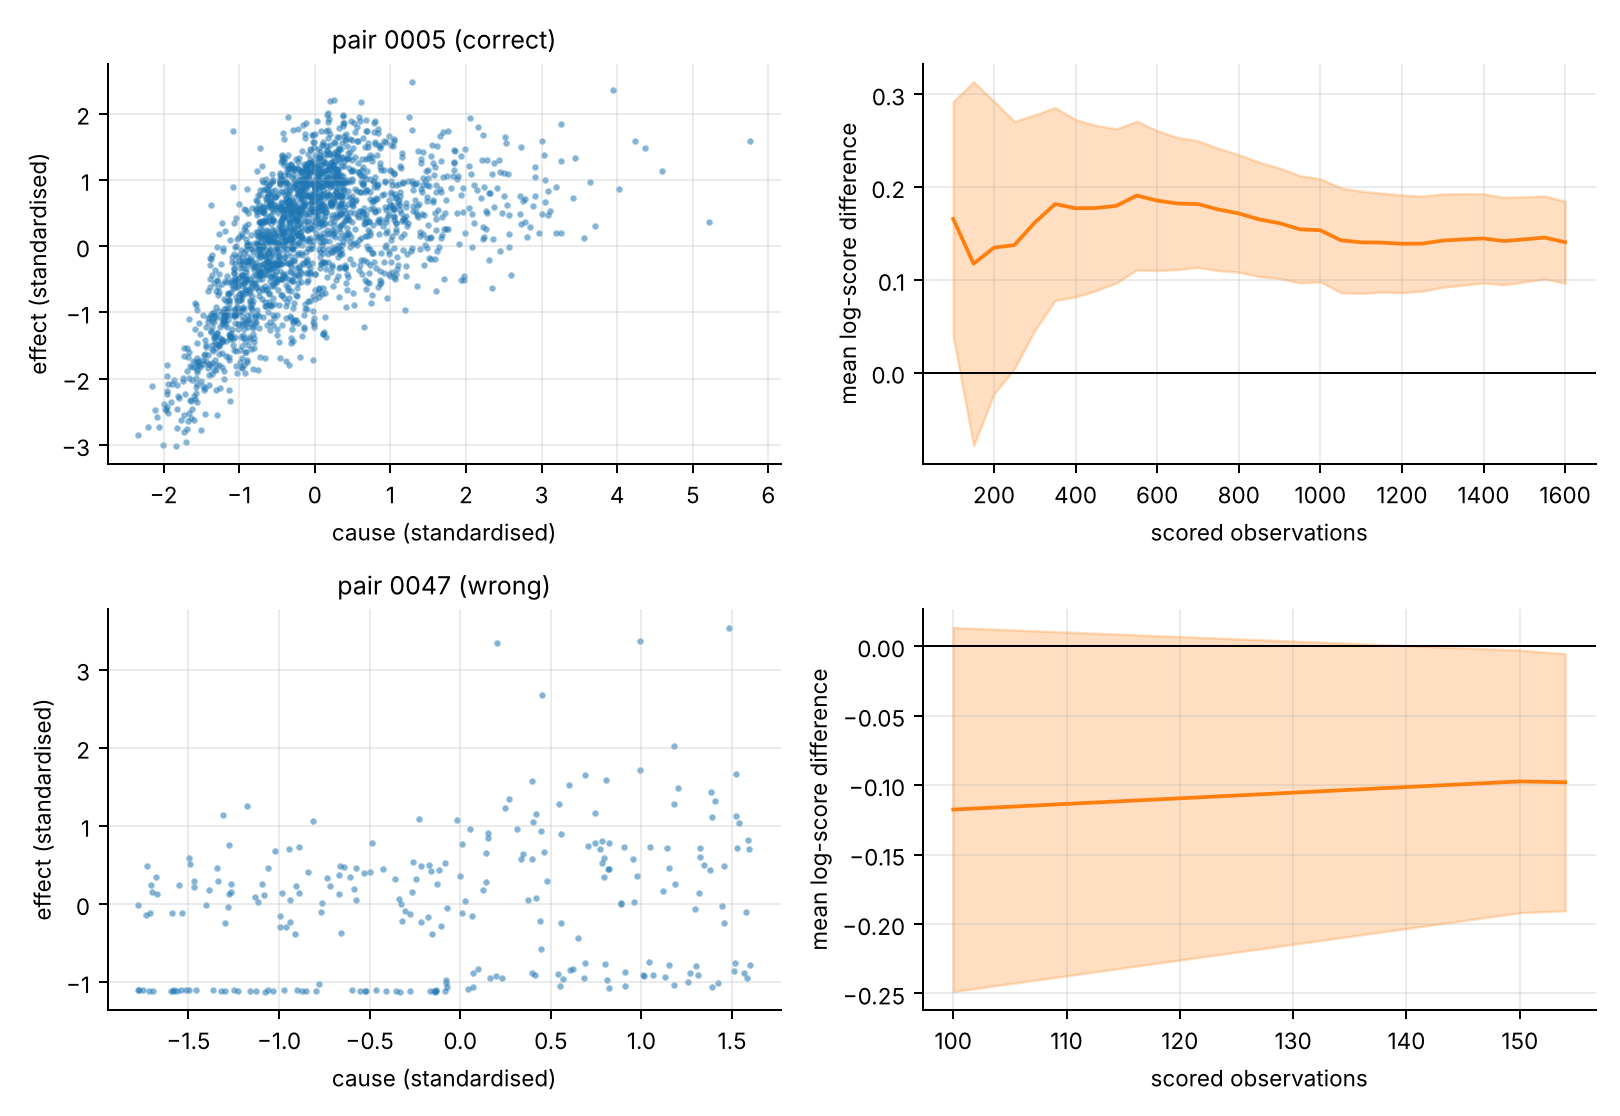
\includegraphics[width=0.85\linewidth]{tuebingen_demo_pairs.png}
\caption{Tübingen pairs~5 (top) and~47 (bottom): scatter plot and confidence
sequence for the running mean log-score difference under the constant-scale
class; a lower end above zero certifies the true direction.}\label{fig:tuebingen}
\end{figure}

\subsection{Real physical data with a known graph: the Causal Chambers}
\label{sec:exp-chamber}

The Causal Chambers \citep{gamella2025chamber} are two physical devices, a wind
tunnel and a light tunnel, whose causal graphs are known from the construction of
the devices and which provide real measurements. We used two recorded
experiments in which the actuators are randomised, chosen before any result was
seen: the wind tunnel with random intake loads ($10$ varying variables, $8$ true
edges among them) and the light tunnel with uniform inputs ($20$ variables, $39$
true edges). A third experiment, the wind tunnel with random
loads on both fans, was dropped before running because the two load variables
are identical in the recording, so the two nodes cannot be told apart. Variables
are the nodes of the chamber graph with at least $20$ distinct values; no node is
hidden. For each dataset we drew $10$ random subsamples of $4000$ rows (rows are
shuffled, to break the serial dependence of the recording) and ran each method
on nested prefixes $n=250,\dots,4000$, as in Section~\ref{sec:exp-monitoring}. The
light tunnel recording has $10000$ rows, so its ten subsamples overlap heavily and
are not independent; counts out of ten there are indicative only.

\paragraph{Linear certificate and comparators.} With the linear
certificate at $k=2$, and with all four comparators, a false edge (an edge of
the algorithm's output that is not an edge of the chamber graph) was reported in
every one of the $10$ subsamples of both devices (rows ``strict'' of
Table~\ref{tab:chamber}). CERT-CD's precision at $n=4000$ was $0.40$ and
$0.41$, similar to PC's, and DirectLiNGAM was the most accurate on the light
tunnel ($0.79$ precision, $0.59$ recall). These results motivated the changes below, so what follows is a
redesign made after seeing these data, not a test on fresh ones.

\paragraph{Sources of the false edges.}
Inspecting the persistent false edges showed three things. First, in the light
tunnel the separator of $\mathrm{ir}_1$ from $\mathrm{ir}_2$ is the five parents of $\mathrm{ir}_1$,
larger than $k=2$, so Assumption~\ref{ass:sep} fails; raising $k$ to $3$ removes
all but three pairs (the three infrared and visible sensor pairs described below). Second, the mechanisms are nonlinear, which the nonparametric
primitive of Section~\ref{sec:npprimitive} handles. Third, some pairs the graph
calls non-adjacent are dependent given the graph's own separating set. To make this
precise without using any of the algorithms under test, we computed, for every
non-adjacent pair, the generalised covariance statistic given the parents of the
non-descendant (additive spline regression) on up to $20000$ rows (the whole
recording, $10000$ rows, in the light tunnel), and call the pairs with $|z|>5$ the
\emph{reference set} $V$. It has $11$ pairs in the wind tunnel: the six pairs of
pressure sensors, which are mutually dependent given their parents with residual
correlation $0.999$, the two rotation speeds ($z=11$), and four pairs of the intake
rotation speed with a pressure sensor ($|z|\approx5.6$, residual correlation about
$-0.03$, close to the cutoff). It has $5$ in the light tunnel: three pairs of the
infrared and visible sensors of the same unit (residual correlation $0.75$ to $0.80$)
and two pairs with $|z|\approx6$ and residual correlation about $-0.07$. These are dependences that the graph cannot explain, plausibly a
shared source or drift that the graph does not contain. A certified edge that is
neither a graph edge nor in $V$ is called a \emph{false edge, adjusted}; the
scoring is partly circular for any method that detects conditional dependence
with large $n$, and we report both versions.

\begin{table}[t]
\caption{Causal Chambers, $10$ subsamples of $4000$ rows each. Columns: ``ever'', subsamples (of $10$) with a false edge,
adjusted for $V$, at some sample size; ``adj.'', false edges per subsample at
$n=4000$, counting a certified pair as correct if it is a graph edge or in the
reference set $V$; ``strict'', the same counting graph edges only; ``rec.'', recall of the graph edges ($8$ and $39$). Wind tunnel: $d=10$, $|V|=11$;
light tunnel: $d=20$, $|V|=5$. The CERT-CD variants have orientation off.}
\label{tab:chamber}
\small
\setlength{\tabcolsep}{3pt}
\scriptsize\setlength{\tabcolsep}{2pt}
\begin{tabular}{@{}lcccccccc@{}}
\toprule
 & \multicolumn{4}{c}{wind tunnel} & \multicolumn{4}{c}{light tunnel}\\
Method & ever & adj. & strict & rec. & ever & adj. & strict & rec.\\
\midrule
CERT-CD nonparam., $k=3$ & 1 & 0.1 & 5.9 & 0.12 & 0 & 0.0 & 3.0 & 0.18\\
CERT-CD lin., $k=3$ & 10 & 1.1 & 3.7 & 0.39 & 4 & 0.4 & 3.5 & 0.18\\
CERT-CD nonparam., $k=2$ & 1 & 0.2 & 6.2 & 0.12 & 10 & 5.6 & 9.6 & 0.19\\
CERT-CD lin., $k=2$ & 10 & 1.1 & 4.6 & 0.39 & 10 & 5.9 & 9.9 & 0.18\\
PC, $\alpha=0.05$ & 10 & 2.0 & 7.9 & 0.53 & 10 & 7.9 & 11.9 & 0.24\\
PC, $\alpha=0.01$ & 10 & 1.8 & 7.2 & 0.44 & 10 & 6.4 & 10.4 & 0.22\\
GES-BIC & 10 & 8.3 & 16.8 & 0.69 & 10 & 8.9 & 12.9 & 0.60\\
DirectLiNGAM & 10 & 4.6 & 10.8 & 0.61 & 10 & 2.9 & 6.1 & 0.59\\
\bottomrule
\end{tabular}
\end{table}

\paragraph{Redesigned certificate.} With the nonparametric primitive and
$k=3$, the adjusted count is $1$ of $10$ subsamples in the wind tunnel
(Wilson $[0.018,0.404]$, $0.1$ false edges per subsample) and $0$ of $10$ in the light tunnel
($[0,0.278]$). In the light tunnel every other configuration in the table is at
$10$ of $10$ except the linear certificate at $k=3$ ($4$ of $10$); in the wind tunnel
every other configuration is at $10$ of $10$ except the nonparametric certificate at
$k=2$ ($1$ of $10$). The nonparametric certificate
certifies $10.1$ edges per subsample in the light tunnel, of which about $7$ are graph edges and
$3$ are pairs of $V$, and its recall of the graph edges is only $0.12$ and
$0.18$. The strict count remains $10$ of $10$ because the pairs of $V$ are
certified, which is the intended behaviour for pairs whose dependence the
graph does not explain, but it means that against the graph alone CERT-CD still
reports false edges. The baselines are scored on the same subsamples; PC, GES and
DirectLiNGAM were run with their usual settings and were not given a larger
conditioning order or a nonparametric test.

\paragraph{Untouched recordings.} Because the choices above were made after seeing
the first two recordings, we froze the algorithms and ran them on recordings that
had not been used (a pre-specified rule: all $15$ random-walk runs of the wind
tunnel with at least $8000$ rows, the pressure-control experiment of the wind
tunnel, and the three light-tunnel walk experiments, $19$ recordings; the
sizes of the graphs are $10$ to $20$ nodes and $18$ to $39$ edges). Each recording
was shuffled and split in halves; the algorithms monitored $4000$ rows of one half
and the reference set $V$ was built on the other half, so that $V$ does not depend on the
monitored rows. Table~\ref{tab:fresh} and the text report what happened.

\begin{table}[t]
\caption{Untouched Causal Chamber recordings. For each group: recordings in which a false
edge was reported at some sample size, adjusted for the reference set $V$ (strict, graph
edges only, in parentheses), false edges per recording at $n=4000$ (adjusted) and recall of
the graph edges. Wind tunnel walks: $15$ recordings, $16$ nodes, $26$ edges, $31$ reference
pairs on average; pressure control: $1$, $11$ nodes, $18$ edges; light tunnel walks: $3$,
$13$ nodes on average, $26$ edges, $14$ reference pairs.}\label{tab:fresh}
\footnotesize
\setlength{\tabcolsep}{2pt}
\begin{tabular}{@{}lccccccccc@{}}
\toprule
 & \multicolumn{3}{c}{wind walks ($15$)} & \multicolumn{3}{c}{pressure control ($1$)} & \multicolumn{3}{c}{light walks ($3$)}\\
Method & ever & /run & rec. & ever & /run & rec. & ever & /run & rec.\\
\midrule
CERT-CD nonparam., $k=3$ & 10 (14) & 1.1 & 0.25 & 1 (1) & 1.0 & 0.12 & 1 (3) & 0.3 & 0.24 \\
CERT-CD linear, $k=3$ & 15 (15) & 2.2 & 0.26 & 1 (1) & 1.0 & 0.12 & 0 (3) & 0.0 & 0.17 \\
PC, $\alpha=0.05$ & 15 (15) & 5.9 & 0.42 & 1 (1) & 2.0 & 0.25 & 2 (3) & 4.3 & 0.37 \\
PC, $\alpha=0.01$ & 15 (15) & 4.9 & 0.38 & 1 (1) & 1.0 & 0.25 & 2 (3) & 3.0 & 0.36 \\
GES-BIC & 15 (15) & 25.8 & 0.71 & 1 (1) & 3.0 & 0.62 & 3 (3) & 2.0 & 0.78 \\
DirectLiNGAM & 15 (15) & 24.0 & 0.62 & 1 (1) & 4.0 & 0.56 & 2 (3) & 3.0 & 0.74 \\
PC, nonparam.\ test, $\alpha=0.05$ & 15 (15) & 6.0 & 0.48 & 1 (1) & 5.0 & 0.31 & 2 (3) & 1.7 & 0.49 \\
PC, nonparam.\ test, $\alpha=0.01$ & 15 (15) & 4.5 & 0.41 & 1 (1) & 3.0 & 0.25 & 2 (3) & 2.7 & 0.48 \\
\bottomrule
\end{tabular}
\end{table}

The guarantee did not hold on these recordings either. The nonparametric
certificate at $k=3$ reported a false edge, adjusted for $V$, in $12$ of the $19$
recordings (and a strict false edge in $18$ of $19$), against $18$ or $19$ of $19$ for the comparators. It
had the fewest false edges per recording in the wind-tunnel walks ($1.1$ against $2.2$
to $25.8$) and, with the linear variant and PC at $\alpha=0.01$, among the fewest in the
other two groups ($1.0$ and $0.3$), but its recall of the graph edges is $0.25$, $0.12$
and $0.24$, below that of every comparator except the linear variant. Counted by precision with
$V$ taken as correct, it certified about $92\%$ of its $14.5$ edges per recording correctly in
the wind-tunnel walks, against $80\%$ for PC at $\alpha=0.01$, $84\%$ for PC with the same
test and about $60\%$ for GES and DirectLiNGAM. We conclude that, on real devices, the
certificate behaves as a conservative edge detector with the fewest false edges among the
methods compared, not as a procedure with a guaranteed false-edge probability.

\paragraph{Direction.} Among the
edges certified by CERT-CD that are true edges, the bivariate agreement
certificate decided $30$ of $31$ in the wind tunnel and $27$ of $70$ in the light
tunnel (the constant-scale class alone $50$ of $70$), and every decision was
correct ($30/30$ and $27/27$). Separately, we applied the certificate to every
true directed edge among the varying variables, each on two random subsamples of
$2000$ rows ($16$ and $78$ pair-runs for the two devices). The
agreement certificate committed on $8$ of $16$ and $23$ of $78$ and was right
every time ($31/31$); the constant-scale class alone committed on $8$ and $40$,
and the location-scale class on $9$ and $25$, also always correctly. The forced
accuracy of the two classes is $0.69$ and $0.69$ in the wind tunnel and $0.74$
and $0.81$ in the light tunnel, against $0.88$ and $1.00$ for RECI, $1.00$ and
$0.92$ for IGCI, $0.38$ and $0.81$ for ANM-HSIC and $0.81$ and $0.77$ for the
pairwise LiNGAM rule. As on the Tübingen pairs, the forced accuracy of
the forecasters is not better than a simple rule, and the certificate is
valuable for what it declines to decide. The causes in these experiments are
uniformly distributed actuators, an easy case for identifiability; the $31$
decisions are $47$ edges analysed twice, and the $30$ and $27$ decisions above pool
the ten subsamples, so neither set is independent.

\subsection{Scope: where the certificates fail}\label{sec:exp-scope}

\paragraph{Assumption violations.} We simulated $200$ datasets of $n=3000$ for each
of four violations at $\alpha=0.05$. In-model there were no false edges and no
wrong arrows. Violating the separator-size premise gave a false edge in
$200/200$ runs and false arrows in $26$; a latent common cause gave a certified
edge in $200/200$ runs, which is a MAG adjacency and not an error in that
sense, with $38$ wrong arrows; nonlinear mechanisms gave false edges in $200/200$
runs and $142$ wrong arrows; Poisson counts gave false edges in $200/200$ runs and
$28$ wrong arrows. The adjacency certificate is valid only for the linear model
with independent errors, and the orientation certificate inside the multivariate
algorithm fails badly under nonlinearity.

\begin{figure}[t]
\centering
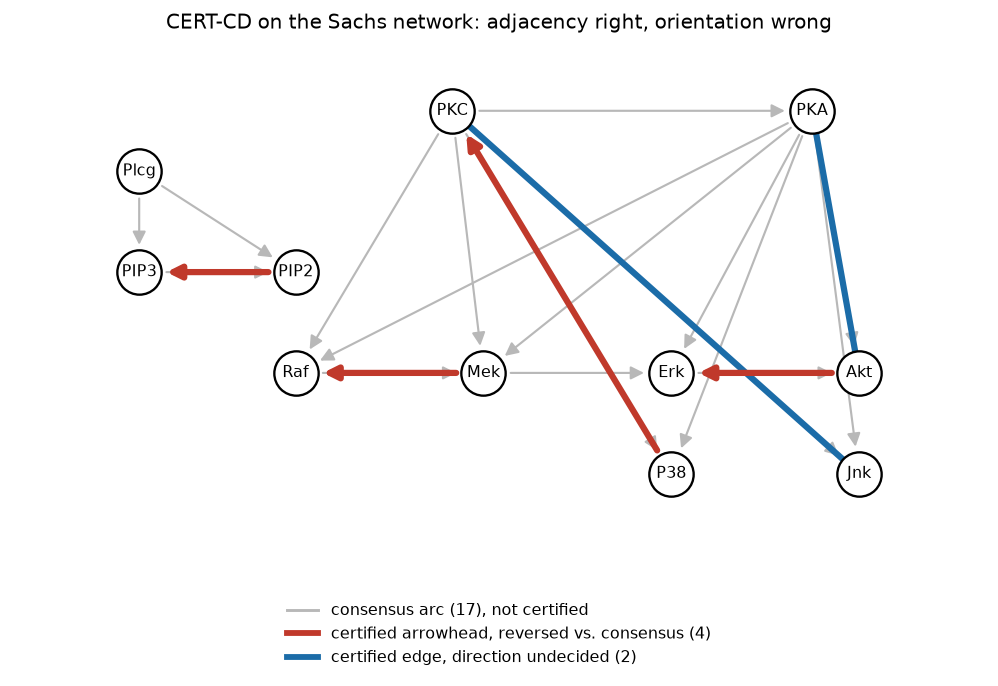
\includegraphics[width=0.8\linewidth]{sachs_network_demo.png}
\caption{Sachs data: certified edges and arrows against the consensus
network.}\label{fig:sachs}
\end{figure}

\paragraph{Sachs protein-signalling data.} The data \citep{sachs2005causal} are
discrete-like, nonlinear and heavy-tailed and sit outside the method's scope,
which is why we report them here. On $853$ cells ($753$ after a $100$-cell
warm-up; Figure~\ref{fig:sachs}) CERT-CD certified $6$ edges among $55$ pairs, all in the consensus
skeleton, left $49$ pairs undecided, and certified $4$ arrowheads, all reversed
relative to the consensus network. PC found $7$ edges, all in the consensus
skeleton. DirectLiNGAM's estimated causal order contradicts the consensus direction on
all six pairs CERT-CD certified (recomputed from the stored order). Consensus directions are themselves contested
\citep{mooij2020joint}, but the certified arrows are confidently
unreliable, and nothing in the output says so. We do not compare with the
iterative protocol of \citet{uehara2026iterative}, whose queries, ground truth
and interaction model differ from ours.


\section{Discussion}\label{sec:discussion}

\paragraph{What is established.} Under monitoring, the adjacency certificate
kept the probability of ever reporting a false edge near $3$--$4\%$ in
random eight-node graphs, where the comparators reached $27\%$ to $100\%$, and
its stated bound is exact in the Gaussian regression model. The orientation
certificate commits rarely and, on the Tübingen pairs under a frozen protocol,
was right on $11$ of the $12$ pairs on which it committed.

\paragraph{Limitations.}
\begin{itemize}
\item \emph{The adjacency bound is asymptotic off the Gaussian model.} The
  null that a partial regression coefficient is zero follows from
  d-separation in a linear model with independent errors, but the primitive is
  exact only for Gaussian regression errors. Section~\ref{sec:exp-primitive}
  measures how far from nominal it is under skewed, heavy-tailed and
  heteroscedastic errors; we have no finite-sample correction. Conditional
  independence testing without a model restriction is impossible
  \citep{shah2020hardness}, so none is to be expected without further
  assumptions.
\item \emph{Power at small samples.} Skeleton recall is $0.21$ at $n=100$ and
  $0.65$ at $n=200$, and at a single large sample size DirectLiNGAM is more
  accurate on the same data. The case for CERT-CD is monitoring, not
  single-sample accuracy.
\item \emph{The order $k$.} Validity needs $k$ at least the size of a separator
  for every non-adjacent pair; $k=0$ and $k=1$ produced false edges in most
  graphs (Section~\ref{sec:exp-ablation}), and nothing in the output warns of it.
\item \emph{Model-class errors in orientation.} On a family with a bimodal cause
  and Gaussian noise, the agreement certificate was wrong on all $5$ pairs it
  decided, because a generalised-Gaussian marginal cannot represent the cause.
\item \emph{Most pairs stay undecided.} About three quarters of the pairs in the
  eight-node experiments are undecided at $n=6400$ because the algorithm
  never certifies absence, and the orientation certificate decided $15\%$ of
  the scorable Tübingen pairs. Certificate-only output trades coverage for
  validity, and a user who needs a complete graph needs a different method.
\item \emph{Predictive fit is not causation.} The orientation certificate
  certifies a better expected log score. It coincides with the causal direction
  under additive-noise or linear non-Gaussian identifiability and under causal
  sufficiency; under confounding it need not, and the multivariate algorithm
  assumes causal sufficiency.
\item \emph{The orientation layer inside the multivariate algorithm is the old
  linear certificate.} Its guarantee is conditional on a linear
  generalised-Gaussian model and fails outside it (Section~\ref{sec:exp-scope}).
  Conditioning the relative-fit forecasters on the frozen block would remove
  this, and is not done here.
\item \emph{Assumed, not checked.} The linear structural model with
  independent errors is an assumption. Residual diagnostics on the warm-up
  prefix can flag gross departures, but they are not part of the guarantee.
\item \emph{Small evidence base for orientation.} The Tübingen result rests on
  $12$ committed pairs out of $80$ scorable, and $22$ of the $102$ pairs were
  too short or discrete to score; the confidence interval on the accuracy is
  wide. The method was designed after an earlier version failed on the same
  data, without tuning on it, and Section~\ref{sec:exp-tuebingen} reports the
  protocol that was fixed.
\item \emph{Domain.} The experiments use continuous data from mostly low-dimensional
  systems. The Sachs data, which are not of this kind, are reported as
  out-of-scope behaviour (Section~\ref{sec:exp-scope}).
\end{itemize}

\section{Conclusion}\label{sec:conclusion}

Asserting a feature of a causal graph only by rejecting a null that is true when
the feature is absent removes the dependence of the false-edge guarantee on
faithfulness and makes the guarantee survive monitoring. In simulation, this
holds at a few percent where deletion-based methods reach most of the graphs,
with the cost that most pairs are left undecided. A predictive-fit orientation
certificate extends the same discipline to direction and committed rarely but
mostly correctly on a standard benchmark. Both certificates are valid only
within their models, and the paper reports where they fail.


\backmatter


\bmhead{Competing interests} The author declares no competing interests.

\bmhead{Funding} This research received no specific grant from any funding
agency in the public, commercial, or not-for-profit sectors.

\bmhead{Ethics approval} Not applicable. The study involves no human
participants or animals. The protein-signalling data analysed in
Section~\ref{sec:exp-scope} are publicly available and were published by
\citet{sachs2005causal}.

\bmhead{Data and code availability} All simulation code, experiment scripts,
random seeds and figure-generating scripts are available at
\url{https://github.com/vinhqdang/SPRINT-CD}. The protein-signalling data of
\citet{sachs2005causal} are redistributed with the \texttt{bnlearn} package
\citep{scutari2010learning} and are downloaded by the experiment script rather
than included in the repository. The Tübingen cause-effect pairs of
Section~\ref{sec:exp-tuebingen} are downloaded on first use from
\url{https://webdav.tuebingen.mpg.de/cause-effect/} and are not redistributed.

\bmhead{Author contributions} The author is solely responsible for all aspects
of this work.

\bmhead{Use of generative AI} A large language model was used in support of
writing this manuscript. The author verified and modified the resulting
content and takes full responsibility for the manuscript in its entirety,
including its claims, derivations, experiments and references.


\begin{appendices}

\section{The safe linear primitive}\label{app:safelinear}

\paragraph{Setup.} Let $y\in\Real^n$ stack the observations of the response
$X_i$, $x$ those of the tested covariate $X_j$, and $W\in\Real^{n\times q}$ the
conditioning block with an intercept, $q=|S|+1$. The model is
$y=W\alpha+\beta x+\varepsilon$, $\varepsilon\sim N(0,\sigma^2I_n)$, with null
$\beta=0$. Let $M=I-W(W^\top W)^{-1}W^\top$ and $\tilde y=My$, $\tilde x=Mx$,
and write $S_{ij}=\tilde x^\top\tilde y$, $S_{ii}=\tilde y^\top\tilde y$,
$S_{jj}=\tilde x^\top\tilde x$, so that $\hat r^2=S_{ij}^2/(S_{ii}S_{jj})$.

\paragraph{Marginal likelihoods.} The null is invariant under
$y\mapsto\lambda y+Wc$, $\lambda>0$, and the right-Haar prior is
$\pi(\alpha,\sigma)\propto\sigma^{-1}$. Integrating $\alpha$ and $\sigma$ gives
$m_0(y)=C_{n,q}S_{ii}^{-(n-q)/2}$. Under the alternative, put
$\beta\mid\sigma\sim N(0,g\sigma^2)$. Completing the square in $\beta$,
\[
m_1(y)=C_{n,q}(1+gS_{jj})^{-1/2}\Bigl(S_{ii}-\frac{S_{ij}^2}{S_{jj}+g^{-1}}\Bigr)^{-(n-q)/2},
\]
and with $G=gS_{jj}$, $\kappa=G/(1+G)$,
\[
E_n=\frac{m_1}{m_0}=(1+G)^{-1/2}\bigl(1-\kappa\hat r_n^2\bigr)^{-(n-q)/2},
\]
which is~\eqref{eq:safelinear}. The constant $g$ is fixed before the monitored
data arrive, from a discarded warm-up prefix.

\paragraph{Proof of Proposition~\ref{prop:safelinear}.} A Bayes factor with a
right-Haar prior on a group acting on the nuisance parameters of both
hypotheses equals the Bayes factor of the maximal invariant
\citep{berger1998bayes,hendriksen2021optional}. The maximal invariant's law
under the null does not depend on $(\alpha,\sigma)$, so $E_n$ is a ratio of a
density to its null density in the filtration $(\mathcal G_n)$ generated by the
maximal invariants, hence a test martingale there. Ville's inequality gives
$\Prob(\exists n:E_n\ge1/\alpha)\le\alpha$ under every Gaussian null.

\paragraph{The raw-observation filtration.} $(E_n)$ is not a martingale in the
filtration of the raw observations. Take $S=\emptyset$, $g=0.25$ and
$X_{1:2}=Y_{1:2}=(-1,1)$, with the Gram matrix centred. Then $E_2=1$, while
under an i.i.d.\ standard Gaussian independence null the exact conditional
expectation is $\Exp[E_3\mid\Fcal_2]\approx1.083>1$. The guarantee is therefore
the Ville bound on the crossing event, which is what
Propositions~\ref{prop:adjacency} and Theorem~\ref{thm:main} use; it is not a
claim about $\Exp[E_\tau]$ at arbitrary stopping times of the raw filtration.

\section{The linear orientation certificate inside the multivariate algorithm}
\label{app:linear}

Inside the streaming algorithm, direction is certified after the pair's
adjacency, with a sequential universal-inference ratio
\citep{wasserman2020universal}. For a pair $(i,j)$ certified at the stopping time
$T$, let $Z_{ij}$ be a block of conditioning variables fixed at $T$. The
numerator is a generalised-Gaussian linear factorisation $x\to y$ given $Z_{ij}$
fitted sequentially on the past after $T$, with shape in $[0.9,8]$ and a
continuation across the Gaussian boundary of the shape grid; the denominator is
the supremum over the reversed linear factorisation. The observations before
$T$ are discarded. Conditionally on $\Fcal_T$ the later observations are i.i.d.\
and $Z_{ij}$ is a fixed set, so the usual universal-inference argument gives an
e-process for the null that the reversed linear factorisation holds; the union
bound over the $d(d-1)$ ordered pairs uses the fixed family and does not depend
on which hypotheses the run examines. The guarantee is conditional on the linear
generalised-Gaussian model describing the pair given $Z_{ij}$, and it fails
outside it (Section~\ref{sec:exp-scope}). A direction is reported after at least
$80$ post-certification observations.

\section{Inverting the primitive into a confidence sequence}\label{app:cs}

Replacing $y$ by $y-\beta_0x$ gives the process for the null $\beta=\beta_0$,
and the set of $\beta_0$ not rejected at $1/\alpha$ is the interval
\[
\hat\beta\pm\frac{1}{S_{jj}}\sqrt{\frac{\tau(S_{ii}S_{jj}-S_{ij}^2)}{1-\tau}},\qquad
\tau=\frac1\kappa\Bigl[1-\Bigl(\frac{\alpha}{\sqrt{1+G}}\Bigr)^{2/(n-q)}\Bigr],
\]
valid for $0<\tau<1$. Since $\alpha<1$, the term in brackets is positive and
$\tau>0$ for every $n>q$; when $\tau\ge1$ the set is the whole line. The closed
form is checked in the test suite against a numerical inversion over a grid of
$\beta_0$.

\section{Additional experimental detail}\label{app:extra}

\paragraph{Hyperparameters.} Warm-up of $50$ discarded rows for the adjacency
stream; prior standard deviation $0.5$ on the standardised scale
($g=0.25$); $k=2$; adjacency share $\alpha_A/\alpha=0.5$; batch size $250$ in the
graph experiments. For the pair orientation certificate: $\alpha=0.05$,
$\rho$ tuned to $t^\ast=200$, a $60$-observation minimum, warm-up
$\max(100,\lceil0.2n\rceil)$.

\paragraph{Reproduction.} \texttt{python experiments/run\_all.py} reproduces the
adjacency experiments. The scripts \texttt{exp13\_monitoring\_fwer.py},
\texttt{exp14\_tuebingen\_relfit.py}, \texttt{exp15\_primitive\_offmodel.py}
and \texttt{exp16\_pair\_orientation\_sim.py} reproduce the tables of
Section~\ref{sec:experiments}; seeds are fixed in each script and the results
are written to \texttt{results/} as JSON.

\end{appendices}

\bibliography{refs}

\end{document}
